\documentclass{article}
\usepackage{amsmath, amssymb, amsthm} %Math enviornments and symbols
\usepackage[margin=1in]{geometry} % set page margins automatically 
\usepackage{color,soul}% Color and highlighting
%\usepackage[round]{natbib}% Citing references, bibliography
\usepackage{enumitem}% Enumerating
\usepackage{tabularx}% Table environments
\usepackage{hyperref}% Include clickable URLs 
\usepackage{tikz} % Package for producing vector graphics
\usepackage{pgfplots} %Produce high-quality function pots
\pgfplotsset{compat=newest}
\usetikzlibrary{automata} % Tikz library for markov chains
\usepackage{subcaption} % Multiple plots together
\usepackage{algorithm} % For writing pseudocode
\usepackage[noend]{algpseudocode}
\usepackage[utf8]{inputenc}

% Define your title in the Preamble

\title{\LaTeX \, Workshop}
\author{Demetrios Papazaharias}
\date{March 2020}

% User Commands

\newcommand{\condExp}[2]{\mathbf{E}\left[#1|#2\right]}

% End Preamble

% Begin Document
\begin{document}
\maketitle
\begin{abstract}
    This is how you define an abstract.
\end{abstract}

\maketitle

\section{Introduction}\label{sec:Introduction}

In Section \ref{subsec:mathenviornments} we will discuss math environments and user commands. In Section \ref{sec:figures} we will discuss figures. In Section \ref{sec:tables} we will discuss tables. In Section \ref{sec:cites} we will discuss citations. The layout of this section is follows:

\begin{enumerate}
	\item Math Environments
\begin{itemize}
	\item In-line Math 
	\item Equations
	\item Multi-line equations (align environment)
\end{itemize}
	\item  User Commands
\end{enumerate}

\subsection{Math Environments} \label{subsec:mathenviornments}


\subsubsection{In-line Math} \label{subsubsec:inlinemath}

In order to write math symbols within a line you need place your math symbols within dollar signs \$  \$. For example, the penalization coefficient for LASSO is $\lambda = 0.5$. 

\subsubsection{Display Math}\label{subsubsec:displaymath}

Quickly displaying one line of math

\[
\bar{x} = \dfrac{1}{n}\sum_{i=1}^n x_i
\]

Piecewise functions

\[
\left| x \right| = \begin{cases}
x \quad &x \geq 0\\
-x \quad &x < 0
\end{cases}
\]

Equation environment allows you to label and reference math lines. For example Equation (\ref{eq:product}) represents the product rule.

\begin{equation}
    \nabla(fg) = f \nabla g + g \nabla f \label{eq:product}
\end{equation}

\subsubsection{Multi-line Equations}\label{subsubsec:multiline}

In this section we will write the formulation for the maximum clique problem. Given a graph $G=(V,E)$, a clique $C \subseteq V$ such that $\forall i,j \in C$, $\lbrace i,j \rbrace \in E$. The maximum clique problem seeks the maximum weight or cardinality clique in $G$. For each $i \in V$ we have the following binary variable.

\[
x_i = \begin{cases}
1 \quad \text{if $i$ is in the max clique}\\
0 \quad \text{otherwise}
\end{cases}
\]

 In order to display multiple lines of equations we can use the align environment

\begin{align}
    \max \quad &\sum_{i \in V} w_i x_i &\\
    \text{s.t} \quad &x_i + x_j \leq 1 \quad &\lbrace i, j \rbrace \notin E \label{ineq:maxclique}\\
    &x_i \in \lbrace 0,1 \rbrace \quad &i \in V
\end{align}

Constraint (\ref{ineq:maxclique}) states that for each node pair not connected by a vertex, only one can belong to the maximum clique. If you don't want to see the numbers on the equations just add * after align.

\begin{align*}
    \max \quad &\sum_{i \in V} w_i x_i &\\
	\text{s.t} \quad &x_i + x_j \leq 1 \quad &\lbrace i, j \rbrace \notin E \\
	&x_i \in \lbrace 0,1 \rbrace \quad &i \in V
\end{align*}

\subsection{User Commands}\label{subsec:usercommands}


Some formatting conventions are specific to a research area and are not defined in \LaTeX. For example to typeset the conditional expectation $\mathbf{E}\left[X|N=n\right]$ we type:

\begin{verbatim}
 $\mathbf{E}\left[X|N=n\right]$
\end{verbatim}

If you need to type this equation multiple times it can become cumbersome and make your document a bit difficult to read. With \LaTeX, you can define your own commands in the preamble of your .tex file in order simplify repetitive and complex formatting. The format for defining your own command is:

\begin{verbatim}
\newcommand{\commandname}[number of args]{out}
\end{verbatim}

In the preamble you can place

\begin{verbatim}
\newcommand{\condExp}[2]{\mathbf{E}\left[#1|#2\right]}
\end{verbatim}

To call our newly defined command, we will type

\begin{verbatim}
\[
$\condExp{X}{N=n}$
\]
\end{verbatim}

\[
\condExp{X}{N=n}
\]


\clearpage

\section{Plotting Figures}\label{sec:figures}

Figure \ref{fig:buffalo} show a map of the different districts in Buffalo.
\begin{figure}[h]
    \centering
    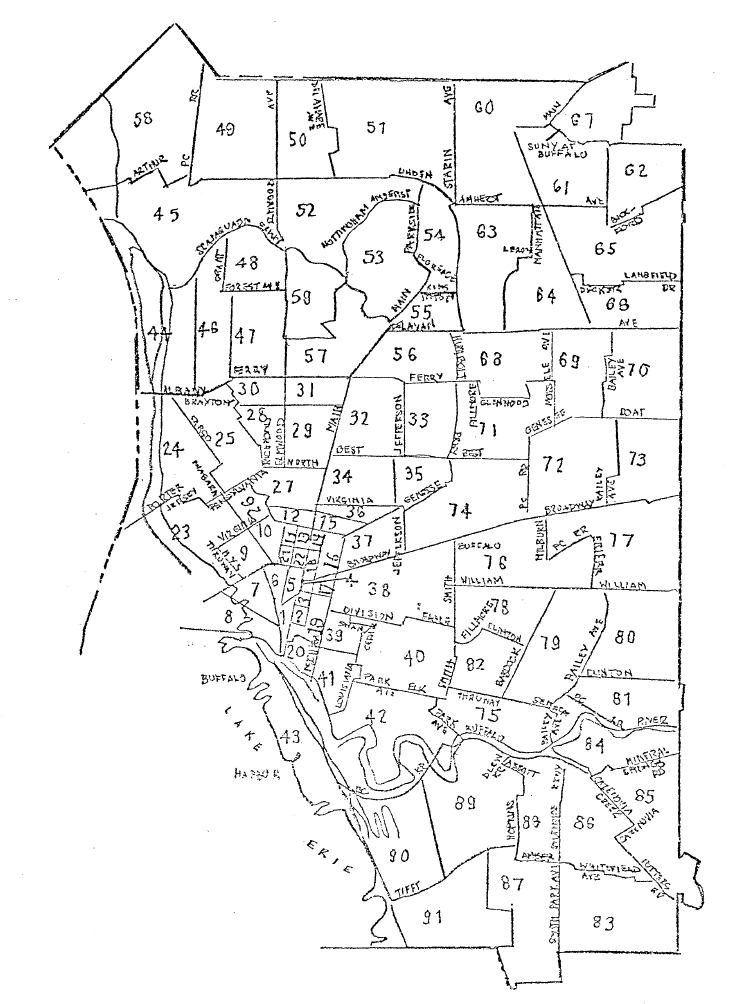
\includegraphics[scale=0.6]{../img/BuffaloMap}
    \caption{Map of Buffalo}
    \label{fig:buffalo}
\end{figure}

\subsection{Multiple Plots}\label{subsec:multiplot}

\begin{minipage}{\textwidth}
	\begin{minipage}[b]{0.5\textwidth}
		\centering
		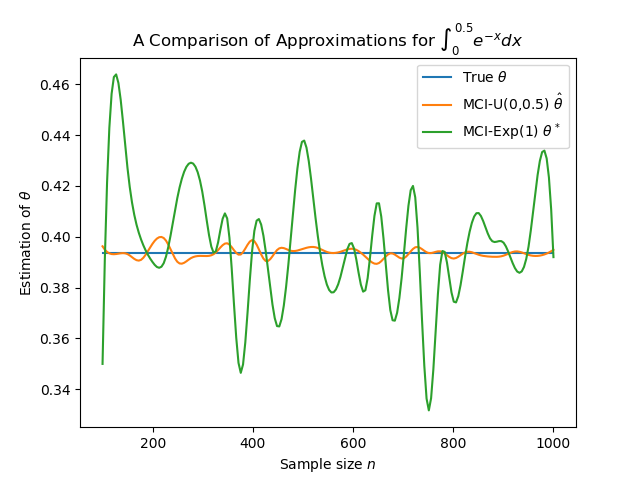
\includegraphics[scale=0.55]{../img/MCI_Results}
		\captionof{figure}{SOM Plot}
		\label{fig:somsubplot}
	\end{minipage}
	\begin{minipage}[b]{0.5\textwidth}
		\centering
		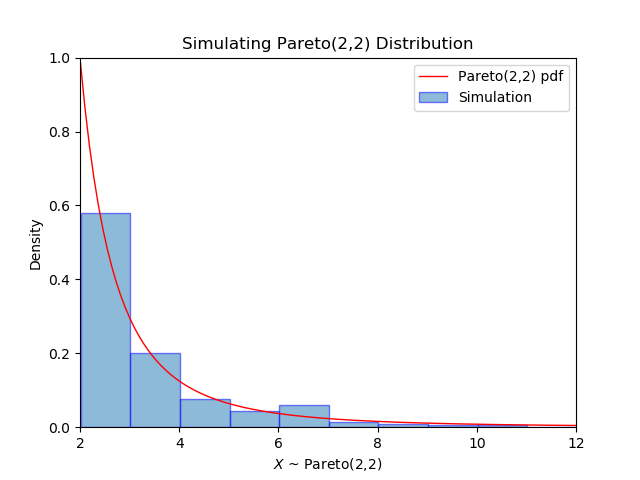
\includegraphics[scale=0.55]{../img/pareto}
		\captionof{figure}{PCA Plot}
		\label{fig:pcasubplot}
	\end{minipage}
\end{minipage}

\subsection{Tikz Picture}\label{subsec:tikz}

Suppose we want to draw the following transition matrix as a Markov Chain

\[
\mathbb{P} = \begin{bmatrix}
0.5 & 0.5 & 0\\
0.5 & 0 & 0.5\\
0 & 1 & 0
\end{bmatrix}
\]

\begin{figure}[h]
	\centering
	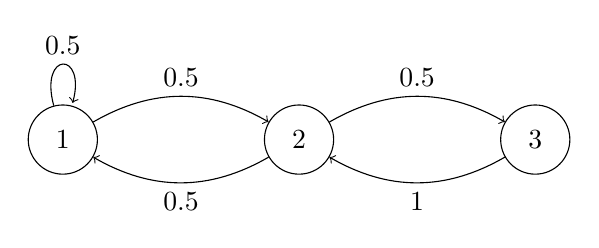
\begin{tikzpicture}[auto, node distance=3cm]
	\node (1) [state] {1};
	\node (2) [state, right of= 1] {2};
	\node (3) [state, right of= 2] {3};
	\path[->]
	% From Node 1
	(1) edge [loop above]  node [above] {0.5} (1)
	(1) edge [bend left]  node [above] {0.5} (2)
	% From Node 2
	(2) edge [bend left] node [below] {0.5} (1)
	(2) edge [bend left] node [above] {0.5} (3)
	% From Node 3
	(3) edge [bend left] node [below] {1} (2);
	\end{tikzpicture}
\end{figure}


\section{Tables}\label{sec:tables}

For constructing tables in \LaTeX, I highly recommend creating tables in Excel and using this webstie: \url{https://www.tablesgenerator.com/latex_tables} to generate the code for those tables. We will create the table from \texttt{table.xlsx}.


\begin{table}[h]
	\centering
	\begin{tabular}{|c|l|l|r|}
		\hline & A & B & C\\
		\hline High & 25 & 10 & 5\\
		\hline Mid & 30 & 15 & 8\\
		\hline Low & 35 & 20 & 10\\
		\hline
	\end{tabular}
	\caption{Table 1}
	\label{tab:table1}
\end{table}


\section{Citations}\label{sec:cites}

We will learn how to cite in Latex by citing the textbook, \textit{Elements of Statistical Learning}. 

\begin{enumerate}
    \item Create a .bib file to place your BibTeX citations.
    \item Right before end document, place the following code
    \begin{verbatim}
        \bibliographystyle{plain}
        \bibliography{bibliography}
    \end{verbatim}
    For a list of different bibliography styles refer to \url{https://www.overleaf.com/learn/latex/Bibtex_bibliography_styles}
    \item Get your citation, look up Elements of Statistical Learning on Google Scholar
    \item Click on the quotation marks below the article
    \begin{figure}[h]
        \centering
        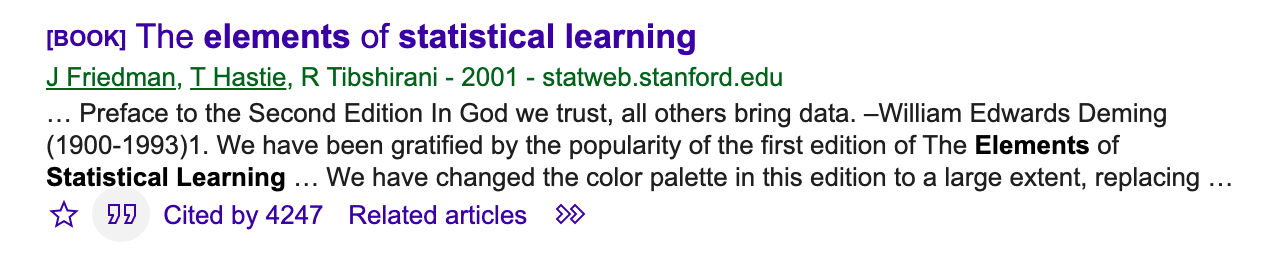
\includegraphics[scale=0.5]{../img/esl.png}
    \end{figure}
    \item Click on BibTeX on the bottom of the window that pops up. You should get the BibTeX citation below. Copy that citation and place into your bibliography.bib file.
    \begin{figure}[h]
        \centering
        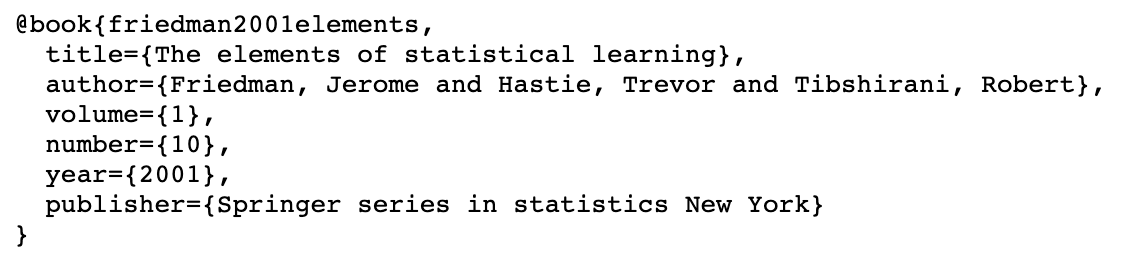
\includegraphics[scale=0.5]{../img/eslcite.png}
    \end{figure}
    \item Once those steps are completed, you can cite our textbook \cite{friedman2001elements}. A reference section with all of the citations used in the document will be generated at the end of the document.
\end{enumerate}


\bibliographystyle{plain}
\bibliography{bibliography}
\end{document}
